
%% CAPÍTULO 1 %%
\chapter{Introducción}

  %% SECCIÓN %%
  \section{Introducción a X}

  Lorem ipsum dolor sit amet, consectetur adipiscing elit. Quisque cursus imperdiet
  pharetra. Donec aliquet sem non leo bibendum cursus. In dictum vel mauris non
  laoreet. Integer in metus magna. Fusce tempus non magna cursus aliquet. Donec
  vitae lobortis felis. Duis tortor sapien, egestas sed leo vitae, sodales hendrerit
  lorem. Nullam sed iaculis lectus, sit amet efficitur purus. In id orci eget lacus
  feugiat vel sed magna.

  Quisque sed lorem et mi pulvinar sollicitudin eleifend non ante. Nullam pretium
  dignissim orci id posuere. Maecenas vehicula ex a enim laoreet, posuere consectetur
  magna rutrum. Suspendisse mi odio, semper quis fringilla sit amet, aliquet ut eros.

  \begin{figure}[!htb]
    \begin{center}
    	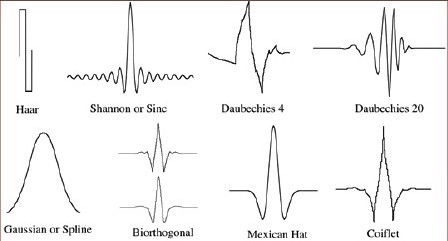
\includegraphics[width=15cm]{./figuras/wavelets.jpg}
    	\caption{Ejemplos de figura}
    \end{center}
    \label{fig:figura}
  \end{figure}

  %% SECCIÓN %%
  \section{Propuesta de Tesis}

  Lorem ipsum dolor sit amet, consectetur adipiscing elit. Quisque cursus imperdiet
  pharetra. Donec aliquet sem non leo bibendum cursus. In dictum vel mauris non
  laoreet. Integer in metus magna. Fusce tempus non magna cursus aliquet. Donec
  vitae lobortis felis. Duis tortor sapien, egestas sed leo vitae, sodales hendrerit
  lorem. Nullam sed iaculis lectus, sit amet efficitur purus. In id orci eget lacus
  feugiat vel sed magna.


  %% SECCIÓN %%
  \section{Contribución del Trabajo}

    sit amet efficitur purus. In id orci eget lacus feugiat vel sed magna.

    \subsection{Aportes}

      Lorem ipsum dolor sit amet, consectetur adipiscing elit. Quisque cursus imperdiet
      pharetra. Donec aliquet sem non leo bibendum cursus. In dictum vel mauris non
      laoreet.

    \subsection{Resultados Esperados}

      Lorem ipsum dolor sit amet, consectetur adipiscing elit. Quisque cursus imperdiet
      pharetra. Donec aliquet sem non leo bibendum cursus. In dictum vel mauris non
      laoreet.

  %% SECCIÓN %%
  \section{Estructura del Trabajo}

    Este trabajo de título se dividirá en los siguientes 4 capítulos, los cuales se describen a continuación:

    \begin{itemize}
      \item \textbf{Capítulo 1: Introducción} \\

      Lorem ipsum dolor sit amet, consectetur adipiscing elit. Quisque cursus imperdiet
      pharetra. Donec aliquet sem non leo bibendum cursus. In dictum vel mauris non
      laoreet.

      \item \textbf{Capítulo 2: Estado del Arte} \\

      Lorem ipsum dolor sit amet, consectetur adipiscing elit. Quisque cursus imperdiet
      pharetra. Donec aliquet sem non leo bibendum cursus. In dictum vel mauris non
      laoreet.

      \item \textbf{Capítulo 3: Materiales y Métodos} \\

      Lorem ipsum dolor sit amet, consectetur adipiscing elit. Quisque cursus imperdiet
      pharetra. Donec aliquet sem non leo bibendum cursus. In dictum vel mauris non
      laoreet.

      \item \textbf{Capítulo 4: Resultados Experimentales} \\

      Lorem ipsum dolor sit amet, consectetur adipiscing elit. Quisque cursus imperdiet
      pharetra. Donec aliquet sem non leo bibendum cursus. In dictum vel mauris non
      laoreet.

      \item \textbf{Capítulo 5: Conclusiones y Trabajo a Futuro} \\

      Lorem ipsum dolor sit amet, consectetur adipiscing elit. Quisque cursus imperdiet
      pharetra. Donec aliquet sem non leo bibendum cursus. In dictum vel mauris non
      laoreet.

    \end{itemize}
